\subsection{System On Chip}

\begin{frame}
  \frametitle{System On Chip}
  \begin{itemize}
    \item {\bf Integrated} Processors
  \end{itemize}
\end{frame}

\begin{frame}
  \frametitle{System On Chip}
  \begin{itemize}
    \item Integrated Processors
    \item {\bf Integrated} Solution: key peripherals for your application needs
  \end{itemize}
\end{frame}

\begin{frame}
  \frametitle{System On Chip}
  \begin{itemize}
    \item Integrated Processors
    \item Integrated Solution: key peripherals for your application needs
  \item {\bf SoC}
  \end{itemize}
\end{frame}

\begin{frame}
  \frametitle{SoC Overview}
  \begin{center}
    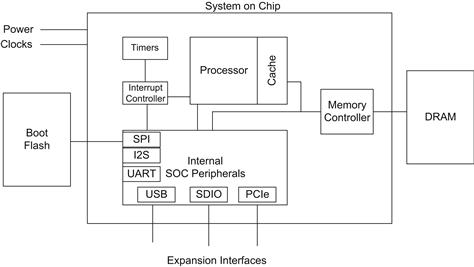
\includegraphics[width=0.9\textwidth]{slides/te5009-embedded-architecture-soc/SoC.jpg}\\
  \end{center}
\end{frame}

\begin{frame}
  \frametitle{CPU}
  \begin{itemize}
    \item {\bf CISC}: Complex Instruction Set Computing
    \item {\bf RISC}: Reduced Instruction Set Computing
  \end{itemize}
\end{frame}

\begin{frame}
  \frametitle{CPU}
  \begin{itemize}
    \item CISC emphasizes {\bf hardware} complexity
    \item RISC emphasizes {\bf compiler} complexity
  \end{itemize}
\end{frame}

\begin{frame}
  \frametitle{CISC vs. RISC}
  \begin{center}
    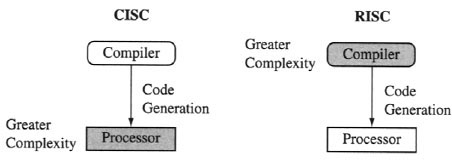
\includegraphics[width=0.7\textwidth]{slides/te5009-embedded-architecture-soc/cisc_risc.jpg}\\
  \end{center}
\end{frame}
